
%(BEGIN_QUESTION)
% Copyright 2006, Tony R. Kuphaldt, released under the Creative Commons Attribution License (v 1.0)
% This means you may do almost anything with this work of mine, so long as you give me proper credit

\textit{Stilling wells} er svært nyttig tilbehør til mange typer væskenivåmålere, inkludert flottør og ultralyd.  Men ved måling av væske-væske-grensesnitt må man passe på at stilling well alltid er neddykket:

$$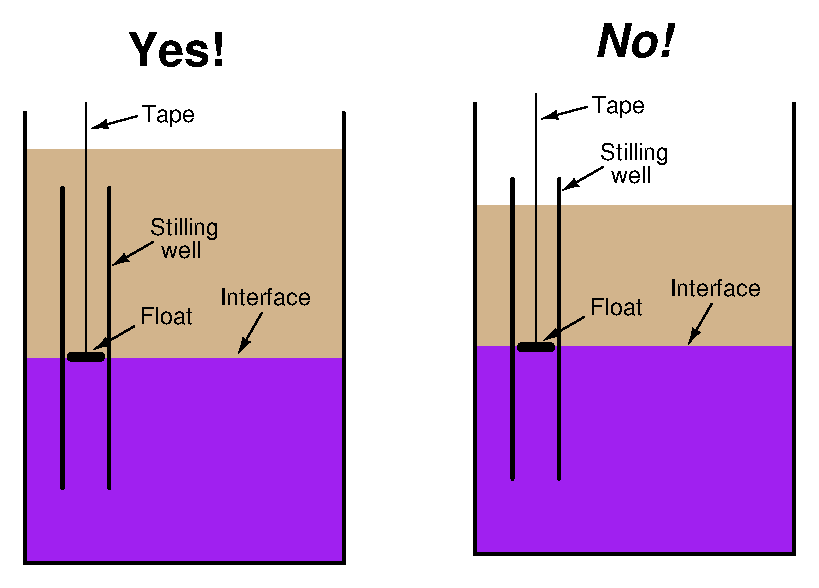
\includegraphics[width=15.5cm]{i00315x01.eps}$$

Forklar hvorfor et stilling well kan brukes i et nivåmålesystem, og hvorfor det må være fullstendig neddykket når det brukes til grensesnittmåling.

\underbar{file i00315}
%(END_QUESTION)





%(BEGIN_ANSWER)

Hvis det ikke er fullstendig neddykket, kan grensesnittnivået inne i røret avvike fra grensesnittnivået i resten av tanken.

%(END_ANSWER)





%(BEGIN_NOTES)

Eksempler på hva som kan skje hvis røret ikke er helt neddykket:

$$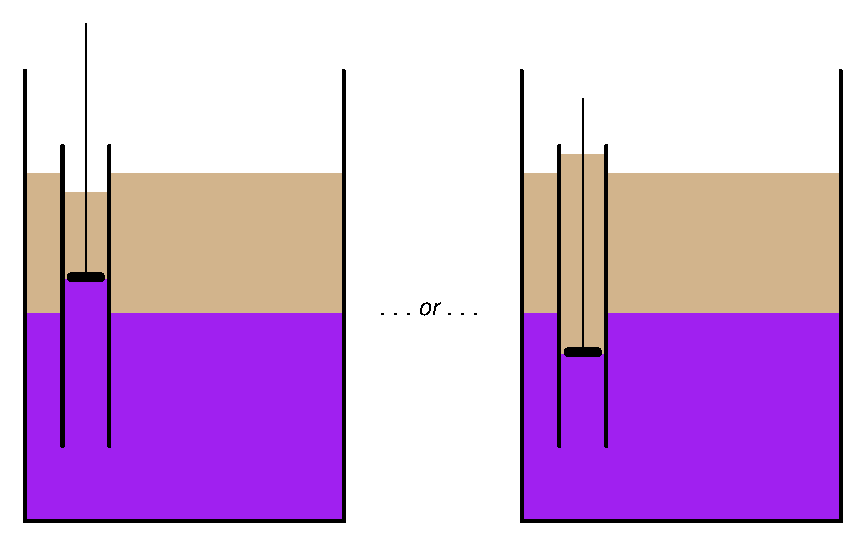
\includegraphics[width=15.5cm]{i00315x02.eps}$$

Uten væsketilgang gjennom toppen av stilling well kan høyden på den lette væskesøylen i røret aldri endres.

%INDEX% Measurement, interface level: use of stilling well

%(END_NOTES)
